\documentclass[a4paper, 14pt]{article}

\usepackage[utf8]{inputenc}
\usepackage[T2A]{fontenc}
\usepackage[english,russian]{babel}
\usepackage{amsthm,amsmath,amsfonts,amssymb}
\usepackage{fullpage}
\usepackage{eufrak}
\usepackage{bbm}
\usepackage{graphicx}
\graphicspath{{images/}}

\begin{document}
\begin{tabbing}
	\hspace{11cm} \= Студент: \= Коротков Фёдор \\ % не забудьте исправить, студент Вы или студентка :)
																									% (а то некоторые забывают)
	\> Группа: \> 2362 \\  % Здесь меняете № группы
	\> Вариант: \> QG \\    % А здесь меняете № варианта
	\> Дата: \> \today     % А вот здесь ничего не меняем!!!
\end{tabbing}
\hrule
\vspace{1cm}
\newcommand{\problemset}[1]{
		\begin{center}
			\large #1
		\end{center}
	}
\renewcommand*{\proofname}{Решение}
\problemset{Комбинаторика и теория графов}
\problemset{Индивидуальное домашнее задание №1}


Дано множество $M = \{ 67, 46, 16, 80, 18, 54, 55, 61 \}$ и следующие бинарные отношения на нем:

\begin{itemize}
    \item $F_1(x,y) = 1 \Leftrightarrow \exists z \in M: (x-z)(y-z) < 0$;
    
    \item $F_2(x,y) = 1 \Leftrightarrow x \ge y$ поразрядно;
    
    \item $F_3(x,y) = 1 \Leftrightarrow [\frac{x}{4}]\ = [\frac{y}{4}]\ $;
    \item $F_4(x,y) = 1 \Leftrightarrow x^2 - y^3$ нечетно;
    \item $F_5(x,y) = 1 \Leftrightarrow |x - y| < 5$.
\end{itemize}
\newtheorem{problem}{Задание}

\begin{problem}
Проверить, является ли бинарное отношение -- рефлексивным, арефлексивным, симметричным, асимметричным, антисимметричным, транзитивным.
	
\end{problem}
\begin{itemize}
	    \item $F_1$ является арефлексивным, т.к. $(x-z)(x-z)>0$; симметричным: $(x-z)(y-z)>0 \Leftrightarrow (y-z)(x-z)>0$; нетранзитивным, т.к. есть хотя бы один случай нетранзитивности: например, $F_1(55, 18) = 1, F_1(18, 54) = 1$, но $F_1(55, 54) = 0$; 
            \item $F_2$ является рефлексивным, т.к. $x \ge x$; антисимметричным, т.к. если $x \ge y$ и $y \ge x$, то $x = y$; транзитивным, т.к. (обозначим матрицу бинарного отношения $A$) $A^2 = A$;
            \item $F_3$ является рефлексивным, т.к. $[\frac{x}{4}]\ = [\frac{x}{4}]\ $; симметричным, т.к.  $[\frac{x}{4}]\ = [\frac{y}{4}]\ \Leftrightarrow [\frac{y}{4}]\ = [\frac{x}{4}]\ $; транзитивным, т.к.  $A^2 = A$;
            \item $F_4$ является арефлексивным, т.к. $x^2 - x^3$ всегда четно; симметричным, т.к. получившаяся матрица симметрична (см. Задание 2); нетранзитивным, т.к. есть хотя бы один случай нетранзитивности: например, $F_4(18, 55) = 1, F_4(55, 54) = 1$, но $F_4(18, 54) = 0$;
            \item $F_5$ является рефлексивным, т.к. $0 = |x - x| < 5$; симметричным, т.к. $|x - y| < 5 \Leftrightarrow |y - x| < 5$; транзитивным, т.к. $A^2 = A$.
	\end{itemize}

\begin{problem}
Построить матрицы и графы этих б.о.
	
\end{problem}


\begin{table}[h!]
\centering

\begin{tabular}{|c|c|c|c|c|c|c|c|c|}
    \hline
    $m_i$ & 16 & 18 & 46 & 54 & 55 & 61 & 67 & 80 \\
    \hline
    16 & 0 & 0 & 1 & 1 & 1 & 1 & 1 & 1 \\
    \hline
    18 & 0 & 0 & 0 & 1 & 1 & 1 & 1 & 1 \\
    \hline
    46 & 1 & 0 & 0 & 0 & 1 & 1 & 1 & 1 \\
    \hline
    54 & 1 & 1 & 0 & 0 & 0 & 1 & 1 & 1 \\
    \hline
    55 & 1 & 1 & 1 & 0 & 0 & 0 & 1 & 1 \\
    \hline
    61 & 1 & 1 & 1 & 1 & 0 & 0 & 0 & 1 \\
    \hline
    67 & 1 & 1 & 1 & 1 & 1 & 0 & 0 & 0 \\
    \hline
    80 & 1 & 1 & 1 & 1 & 1 & 1 & 0 & 0 \\
    \hline
\end{tabular}
\caption{Матрица для $F_1$}
\label{Матрица:1}


\end{table}

\begin{figure}
    \centering
    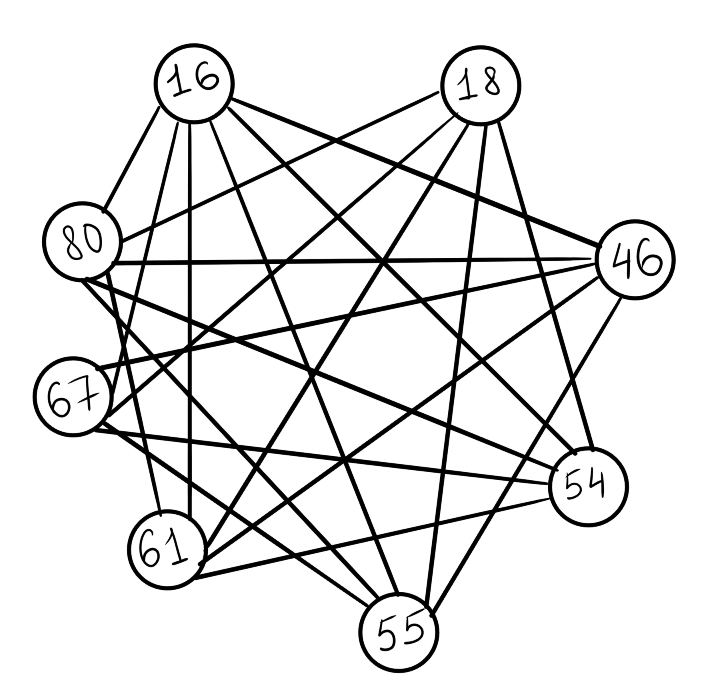
\includegraphics[width=0.4\textwidth]{graph1.png}
    \caption{Граф для $F_1$}
    \label{Рисунок:1}
\end{figure}

\begin{table}
\centering
\begin{tabular}{|c|c|c|c|c|c|c|c|c|}
    \hline
    $m_i$ & 16 & 18 & 46 & 54 & 55 & 61 & 67 & 80 \\
    \hline
    16 & 1 & 0 & 0 & 0 & 0 & 0 & 0 & 0 \\
    \hline
    18 & 1 & 1 & 0 & 0 & 0 & 0 & 0 & 0 \\
    \hline
    46 & 1 & 0 & 1 & 0 & 0 & 0 & 0 & 0 \\
    \hline
    54 & 0 & 0 & 0 & 1 & 0 & 0 & 0 & 0 \\
    \hline
    55 & 0 & 0 & 0 & 1 & 1 & 0 & 0 & 0 \\
    \hline
    61 & 0 & 0 & 0 & 0 & 0 & 1 & 0 & 0 \\
    \hline
    67 & 1 & 0 & 1 & 1 & 1 & 1 & 1 & 0 \\
    \hline
    80 & 0 & 0 & 0 & 0 & 0 & 0 & 0 & 1 \\
    \hline
\end{tabular}
\caption{Матрица для $F_2$}
\label{Матрица:2}
\end{table}

\begin{figure}
    \centering
    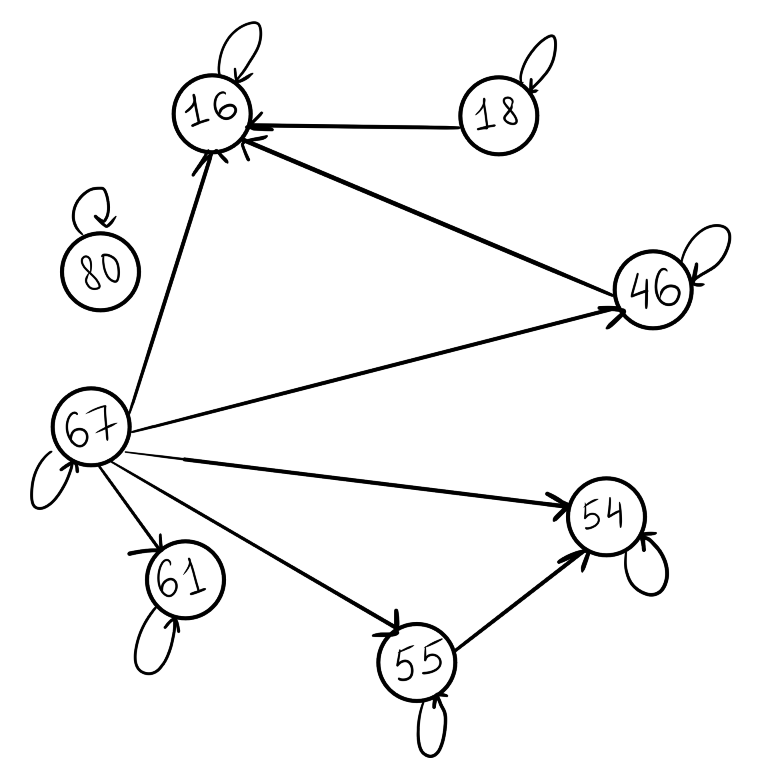
\includegraphics[width=0.4\textwidth]{graph2.png}
    \caption{Граф для $F_2$}
    \label{Рисунок:2}
\end{figure}

\begin{table}
\centering
\begin{tabular}{|c|c|c|c|c|c|c|c|c|}
    \hline
    $m_i$ & 16 & 18 & 46 & 54 & 55 & 61 & 67 & 80 \\
    \hline
    16 & 1 & 1 & 0 & 0 & 0 & 0 & 0 & 0 \\
    \hline
    18 & 1 & 1 & 0 & 0 & 0 & 0 & 0 & 0 \\
    \hline
    46 & 0 & 0 & 1 & 0 & 0 & 0 & 0 & 0 \\
    \hline
    54 & 0 & 0 & 0 & 1 & 1 & 0 & 0 & 0 \\
    \hline
    55 & 0 & 0 & 0 & 1 & 1 & 0 & 0 & 0 \\
    \hline
    61 & 0 & 0 & 0 & 0 & 0 & 1 & 0 & 0 \\
    \hline
    67 & 0 & 0 & 0 & 0 & 0 & 0 & 1 & 0 \\
    \hline
    80 & 0 & 0 & 0 & 0 & 0 & 0 & 0 & 1 \\
    \hline
\end{tabular}
\caption{Матрица для $F_3$}
\label{Матрица:3}
\end{table}

\begin{figure}
    \centering
    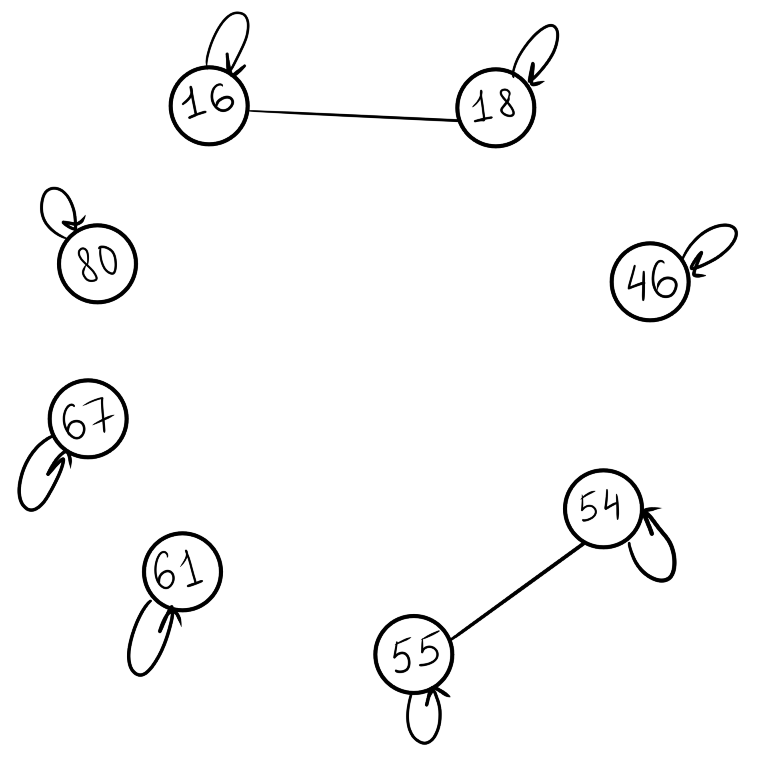
\includegraphics[width=0.4\textwidth]{graph3.png}
    \caption{Граф для $F_3$}
    \label{Рисунок:3}
\end{figure}

\begin{table}
\centering
\begin{tabular}{|c|c|c|c|c|c|c|c|c|}
    \hline
    $m_i$ & 16 & 18 & 46 & 54 & 55 & 61 & 67 & 80 \\
    \hline
    16 & 0 & 0 & 0 & 0 & 1 & 1 & 1 & 0 \\
    \hline
    18 & 0 & 0 & 0 & 0 & 1 & 1 & 1 & 0 \\
    \hline
    46 & 0 & 0 & 0 & 0 & 1 & 1 & 1 & 0 \\
    \hline
    54 & 0 & 0 & 0 & 0 & 1 & 1 & 1 & 0 \\
    \hline
    55 & 1 & 1 & 1 & 1 & 0 & 0 & 0 & 1 \\
    \hline
    61 & 1 & 1 & 1 & 1 & 0 & 0 & 0 & 1 \\
    \hline
    67 & 1 & 1 & 1 & 1 & 0 & 0 & 0 & 1 \\
    \hline
    80 & 0 & 0 & 0 & 0 & 1 & 1 & 1 & 0 \\
    \hline
\end{tabular}
\caption{Матрица для $F_4$}
\label{Матрица:4}
\end{table}

\begin{figure}
    \centering
    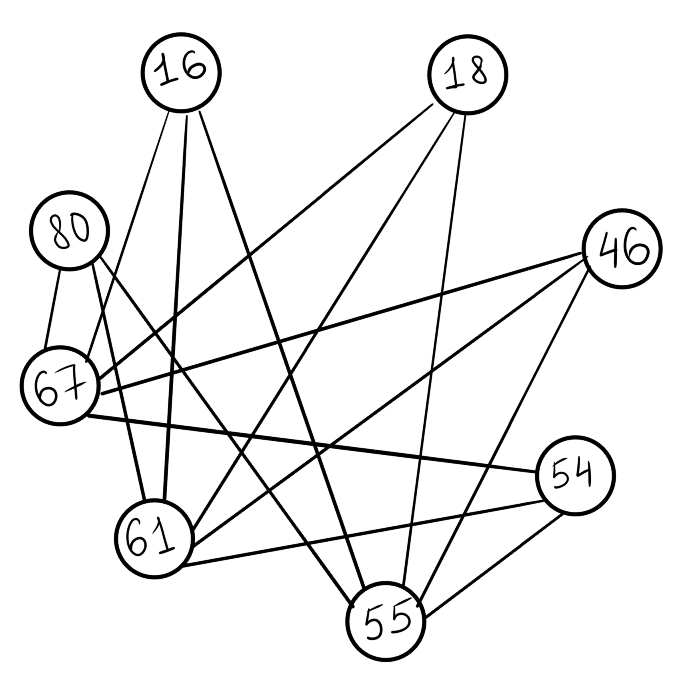
\includegraphics[width=0.4\textwidth]{graph4.png}
    \caption{Граф для $F_4$}
    \label{Рисунок:4}
\end{figure}

\begin{table}[h]
\centering
\begin{tabular}{|c|c|c|c|c|c|c|c|c|}
    \hline
    $m_i$ & 16 & 18 & 46 & 54 & 55 & 61 & 67 & 80 \\
    \hline
    16 & 1 & 1 & 0 & 0 & 0 & 0 & 0 & 0 \\
    \hline
    18 & 1 & 1 & 0 & 0 & 0 & 0 & 0 & 0 \\
    \hline
    46 & 0 & 0 & 1 & 0 & 0 & 0 & 0 & 0 \\
    \hline
    54 & 0 & 0 & 0 & 1 & 1 & 0 & 0 & 0 \\
    \hline
    55 & 0 & 0 & 0 & 1 & 1 & 0 & 0 & 0 \\
    \hline
    61 & 0 & 0 & 0 & 0 & 0 & 1 & 0 & 0 \\
    \hline
    67 & 0 & 0 & 0 & 0 & 0 & 0 & 1 & 0 \\
    \hline
    80 & 0 & 0 & 0 & 0 & 0 & 0 & 0 & 1 \\
    \hline
\end{tabular}
\caption{Матрица для $F_5$}
\label{Матрица:5}
\end{table}

\begin{figure}[h!]
    \centering
    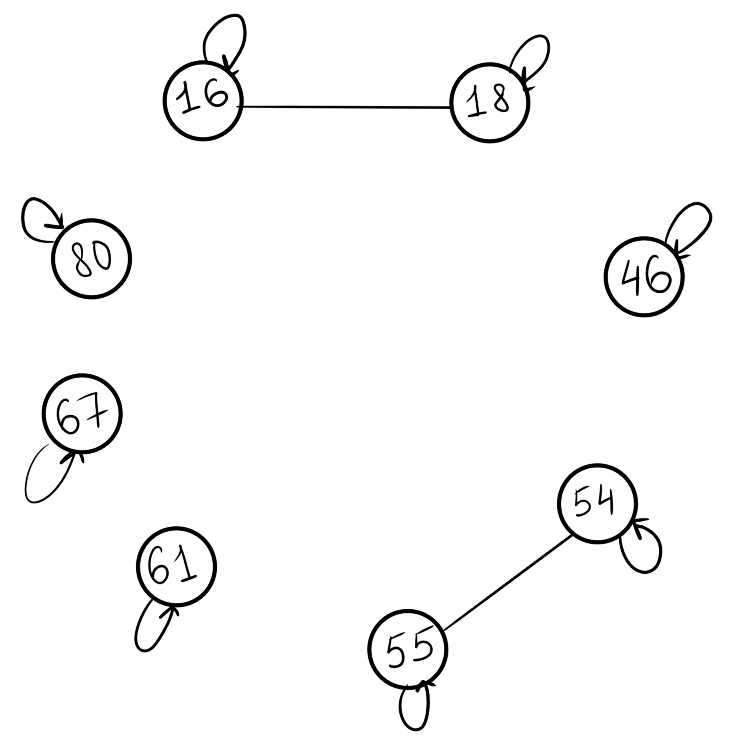
\includegraphics[width=0.4\textwidth]{graph5.png}
    \caption{Граф для $F_5$}
    \label{Рисунок:5}
\end{figure}

\newpage

\begin{problem}
    Определить, являются ли эти б.о. отношениями эквивалентности, частичного порядка, линейного порядка, строгого порядка.
\end{problem}

\begin{itemize}
    \item $F_1$ не является ни одним из типов отношений, т.к. оно арефлексивно, симметрично и нетранзитивно.
    \item $F_2$ является отношением частичного порядка, т.к. оно рефлексивно, антисимметрично и транзитивно. Оно не является отношением линейного порядка, т.к. существуют пары элементов из множества, не связанных этим отношением (например, 18 и 80, 46 и 54).
    \item $F_3$ является отношением эквивалентности, т.к. оно рефлексивно, симметрично и транзитивно.
    \item $F_4$ не является ни одним из типов отношений, т.к. оно арефлексивно, симметрично и нетранзитивно.
    \item $F_5$ является отношением эквивалентности, т.к. оно рефлексивно, симметрично и транзитивно.
\end{itemize}

\begin{problem}
    Для отношений эквивалентности построить классы эквивалентности.
\end{problem}

\begin{itemize}
    \item Классы эквивалентности для $F_3$: $ \{ 16, 18 \}, \{ 54, 55 \},\{ 46 \},\{ 61 \},\{ 67 \},\{ 80 \}$;
    \item Классы эквивалентности для $F_5$: $ \{ 16, 18 \}, \{ 54, 55 \},\{ 46 \},\{ 61 \},\{ 67 \},\{ 80 \}$.
\end{itemize}

\begin{problem}
    Для отношений частичного порядка применить алгоритм топологической сортировки и получить отношение линейного порядка.
\end{problem}

\begin{figure}[h!]
    \centering
    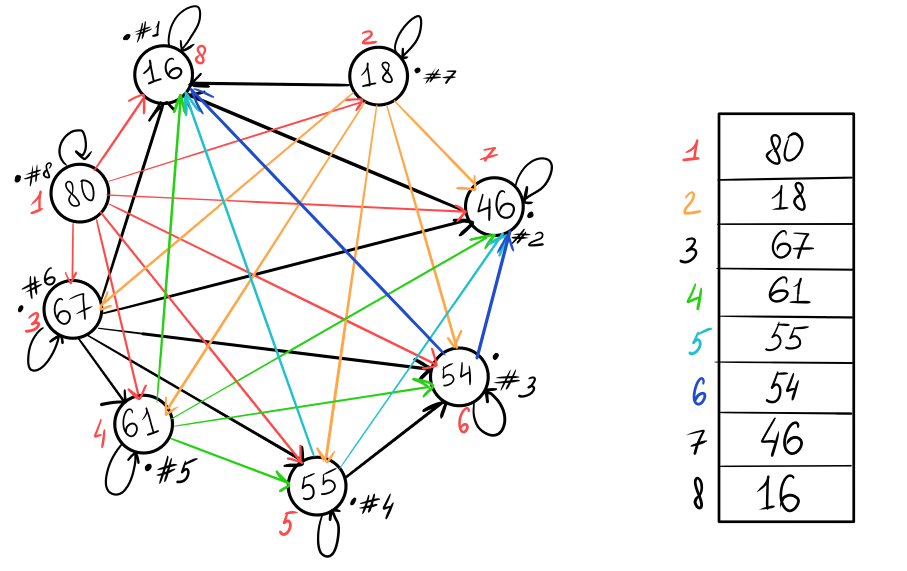
\includegraphics[width=0.8\textwidth]{task5.png}
    \caption{Решение задания 5}
    \label{Рисунок:6}
\end{figure}

\begin{problem}
    Для нетранзитивных отношений построить транзитивное замыкание, используя алгоритм Уоршелла.
\end{problem}
Построим транзитивное замыкание для $F_1$:
\begin{figure}[h!]
    \centering
    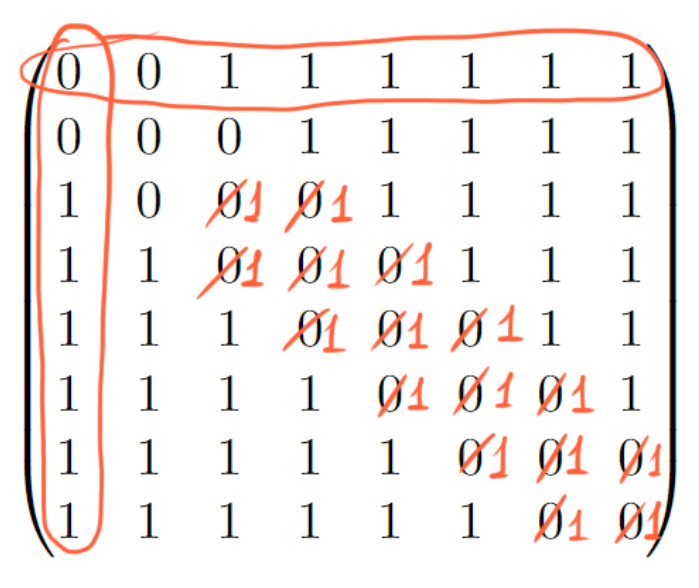
\includegraphics[width=0.3\textwidth]{task6_1.png}
    \caption{Шаг 1}
    \label{Рисунок:7}
\end{figure}
\newpage
На шаге 2 матрица не изменится.
\begin{figure}[h!]
    \centering
    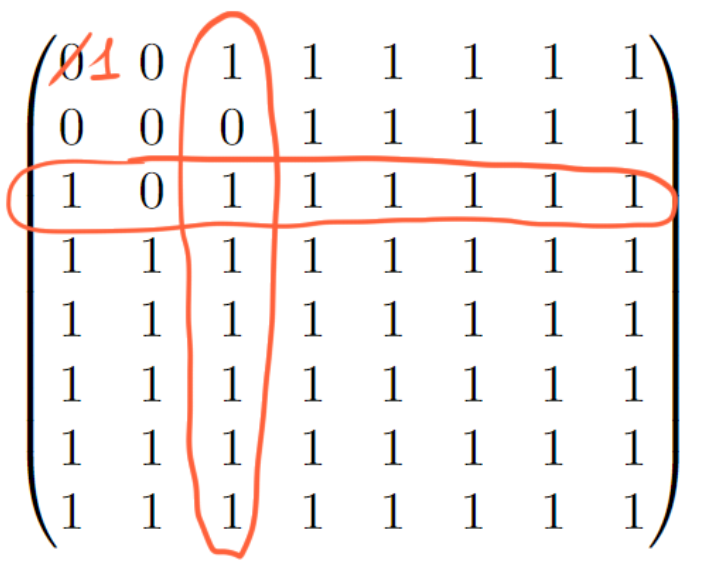
\includegraphics[width=0.3\textwidth]{task6_2.png}
    \caption{Шаг 3}
    \label{Рисунок:8}
\end{figure}
\begin{figure}[h!]
    \centering
    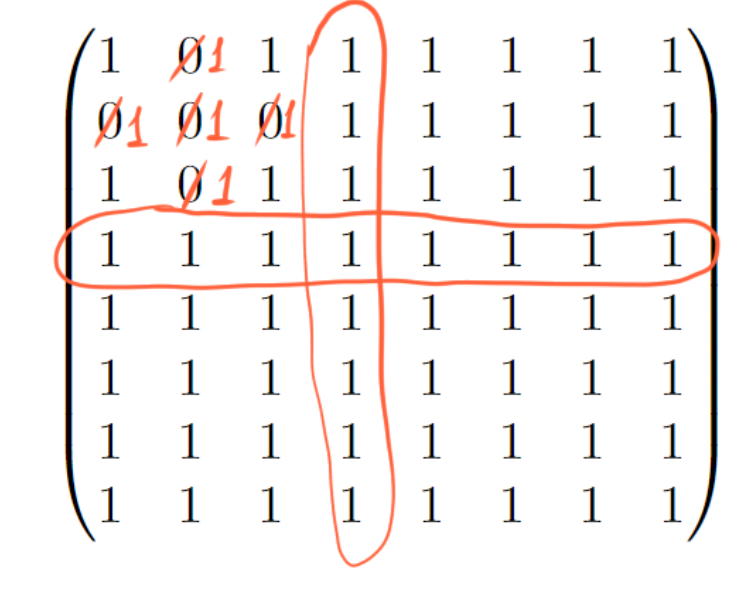
\includegraphics[width=0.3\textwidth]{task6_3.png}
    \caption{Шаг 4}
    \label{Рисунок:9}
\end{figure}
\
$ \\
\\
\text{Ответ: }
\begin{pmatrix}
1 & 1 & 1 & 1 & 1 & 1 & 1 & 1\\
1 & 1 & 1 & 1 & 1 & 1 & 1 & 1\\
1 & 1 & 1 & 1 & 1 & 1 & 1 & 1\\
1 & 1 & 1 & 1 & 1 & 1 & 1 & 1\\
1 & 1 & 1 & 1 & 1 & 1 & 1 & 1\\
1 & 1 & 1 & 1 & 1 & 1 & 1 & 1\\
1 & 1 & 1 & 1 & 1 & 1 & 1 & 1\\
1 & 1 & 1 & 1 & 1 & 1 & 1 & 1\\
\end{pmatrix} \\$

Построим транзитивное замыкание для $F_4$:
\begin{figure}[h!]
    \centering
    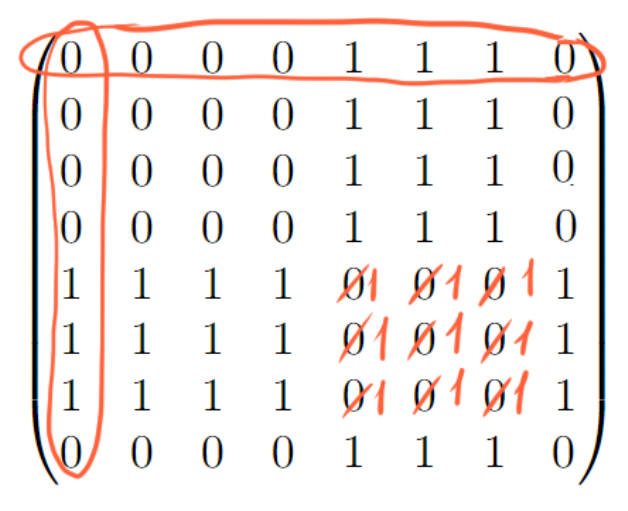
\includegraphics[width=0.3\textwidth]{task6_4.png}
    \caption{Шаг 1}
    \label{Рисунок:7}
\end{figure}
$\\$
На шаге 2, 3 и 4 матрица не изменится.
\begin{figure}[h!]
    \centering
    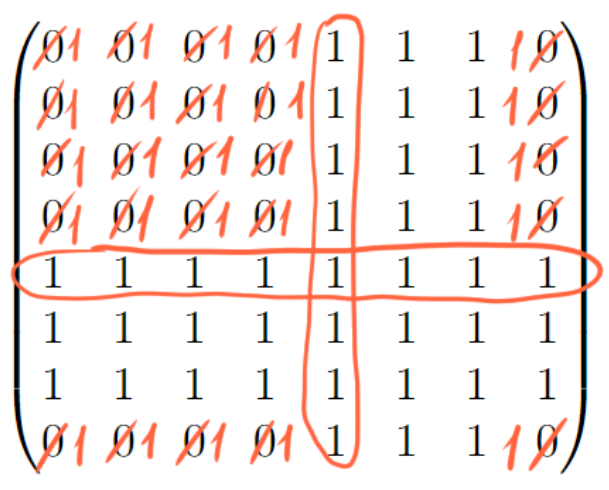
\includegraphics[width=0.3\textwidth]{task6_5.png}
    \caption{Шаг 5}
    \label{Рисунок:8}
\end{figure}
\
$ \\
\\
\text{Ответ: }
\begin{pmatrix}
1 & 1 & 1 & 1 & 1 & 1 & 1 & 1\\
1 & 1 & 1 & 1 & 1 & 1 & 1 & 1\\
1 & 1 & 1 & 1 & 1 & 1 & 1 & 1\\
1 & 1 & 1 & 1 & 1 & 1 & 1 & 1\\
1 & 1 & 1 & 1 & 1 & 1 & 1 & 1\\
1 & 1 & 1 & 1 & 1 & 1 & 1 & 1\\
1 & 1 & 1 & 1 & 1 & 1 & 1 & 1\\
1 & 1 & 1 & 1 & 1 & 1 & 1 & 1\\
\end{pmatrix}$
\end{document}